\documentclass[12pt]{article}

% ---------------------------------------------------------------
% Packages
% ---------------------------------------------------------------
\usepackage[margin=1in]{geometry}
\usepackage{setspace}
\usepackage{amsmath, amssymb}
\usepackage{graphicx}
\usepackage{booktabs}
\usepackage{threeparttable}
\usepackage{caption}
\usepackage{subcaption}
\usepackage{hyperref}
\usepackage{natbib}
\usepackage{authblk}

\setcitestyle{authoryear, open={(}, close={)}}
\onehalfspacing

% ---------------------------------------------------------------
% Title / Authors
% ---------------------------------------------------------------
% Working titles (pick one):
%   "Reading the Storm: Media Attribution of U.S. Climate Disasters, 2000-2024"
%   "Whose Fault Is the Weather? Attribution in Local Newspaper Coverage of Billion-Dollar Disasters"
%   "From Newsprint to Narrative: How U.S. Newspapers Attribute Climate Disasters"

\title{Reading the Storm: Media Attribution of U.S.\ Climate Disasters, 2000--2024}

\author[1]{Hari Gunda}
\author[2]{Michael Price}
\author[3]{Angela Doku}
\author[4]{John List}

\affil[1]{TODO: Affiliation}
\affil[2]{University of Alabama}
\affil[3]{University of Toronto}
\affil[4]{University of Chicago}

\date{\today}

\begin{document}

\maketitle

% ---------------------------------------------------------------
\begin{abstract}
TODO (150--250 words). Motivation: how local and national newspapers
frame the causes of billion-dollar U.S.\ climate disasters --
anthropogenic vs.\ natural/random attribution -- and what drives
variation in that framing. Briefly state data (NOAA Billion-Dollar
Disasters, 2000--2024, matched to newspaper coverage via Google
Custom Search), method (NLP-based Attribution Index at the article
and disaster level), and headline findings (to be filled in).
\end{abstract}

\noindent \textbf{Keywords:} climate change attribution, media framing,
natural language processing, disaster economics

\newpage


% ===================================================================
\section{Introduction}
% ===================================================================

TODO: Motivate the question --- do U.S.\ newspapers attribute
billion-dollar weather/climate disasters to anthropogenic climate
change, or frame them as natural/random variation? Why does this
matter (public risk perception, policy salience, insurance markets,
disaster preparedness)? Preview data, method, and main results.
Outline the rest of the paper.


% ===================================================================
\section{Related Literature}
% ===================================================================

TODO: Position relative to (i) climate communication / media framing
literature, (ii) economics of natural disasters and salience,
(iii) text-as-data / NLP methods in economics, (iv) political economy
of climate policy and local media markets.


% ===================================================================
\section{Data}
\label{sec:data}
% ===================================================================

\subsection{NOAA Billion-Dollar Disasters Dataset}

The sample is drawn from NOAA's Weather and Climate Billion-Dollar
Disasters dataset, restricted to U.S.\ events occurring between 2000
and 2024 (313 events). Each event is characterized by a disaster type
(Severe Storm, Tropical Cyclone, Flooding, Drought, Wildfire, Winter
Storm, or Freeze), a begin and end date, the set of affected states,
CPI-adjusted and unadjusted cost (in millions of 2024 dollars), and a
fatality count. Severe storms are the most common event type (179 of
313 events), followed by tropical cyclones (48), flooding (30),
drought (21), wildfire (19), winter storm (13), and freeze (3). Total
CPI-adjusted damages across the sample exceed \$2.36 trillion, with a
median event cost of \$2.4 billion (mean \$7.5 billion, driven by a
right tail of extreme events up to \$201.3 billion); total reported
fatalities across all events are 10,849.

\subsection{Newspaper Coverage Data}

\paragraph{Newspaper universe.} The candidate universe of outlets is
drawn from the Access World News (AWN) database, which lists 3,647
U.S.\ newspapers and wire services with associated city, state, and
language metadata. Of these, 970 had no listed website and were
excluded. The remaining outlets were passed through an automated
verification pipeline that attempted to resolve and HTTP-check each
listed URL (classifying each as verified, verified via HTTP-only,
or unverified with a status code/reason); 899 outlets ultimately
produced a usable, live domain.

\paragraph{Programmable Search Engine (PSE) construction.} The 899
verified domains were partitioned into 18 regional Google
Programmable Search Engines (PSEs), grouped by the states each outlet
primarily serves, plus a 19th ``National'' PSE covering major national
and wire outlets (e.g., the \emph{New York Times}, \emph{Washington
Post}, CNN, AP, NPR, USA Today) that are relevant regardless of event
geography. Each of the 313 disaster events is mapped to the subset of
regional PSEs corresponding to its affected states (plus the National
PSE), so that searches are restricted to outlets plausibly covering
that event's geography.

\paragraph{Collection pipeline.} For each event, queries combining the
disaster name/type and date window are issued against the relevant
PSE subset via the Google Custom Search JSON API. Candidate results
are filtered on (i) a date window around the event's begin/end dates
(with retrospective coverage allowed up to the start of the next event
of the same type, where applicable), (ii) geographic relevance --
results must reference a place name consistent with the event's
affected states or broader region, and (iii) disaster-type/keyword
relevance. Up to 30 candidate articles are retained per event. The
full collection run returned 1,694 candidate articles across the 313
events: 237 events (75.7\%) returned at least one candidate article
(mean 5.4 articles per event among events with any coverage; 76
events returned none). Of the 1,694 candidate articles, 911 (53.8\%)
are from outlets on the National PSE list and 783 (46.2\%) are from
regional/local outlets. These candidate articles are then passed
through the relevance-screening and attribution-coding procedure
described in Section~\ref{sec:methods}.

\subsection{Constructing the Attribution Index}
\label{sec:attribution_index_data}

Each of the 1,694 candidate articles is first screened for
\emph{relevance} -- whether it substantively discusses the specific
NOAA-listed event it was retrieved for (correct disaster, geography,
and time window), versus being off-topic, ambiguous (\texttt{Borderline}),
or unusable (\texttt{Trash}). Only articles coded \texttt{Relevant}
proceed to attribution coding.

Each relevant article is then assigned to one of five categories
describing how it frames the causal origin of the event, with an
associated numeric score $a_{i,d} \in \{-1, 0, 0.5, 1\}$:

\begin{table}[ht]
\centering
\caption{Attribution Coding Categories}
\label{tab:attribution_categories}
\begin{threeparttable}
\begin{tabular}{clc}
\toprule
Code & Description & Score \\
\midrule
A & Explicit anthropogenic climate-change attribution & $+1.0$ \\
B & Hedged / contextual climate mention & $+0.5$ \\
C & No causal attribution (pure event reporting) & $0.0$ \\
D & Explicit non-climate attribution (natural variability or other human causes) & $-1.0$ \\
E & Mixed / contested framing & $0.0$ (flagged) \\
\bottomrule
\end{tabular}
\begin{tablenotes}
\small
\item Notes: Full category definitions, decision rules, and example
language are given in the project codebook
(\texttt{paper/attribution\_codebook.md}). Category E receives the
same numeric score as C but is separately flagged as
\emph{contested} when computing disaster-level dispersion.
\end{tablenotes}
\end{threeparttable}
\end{table}

Article-level scores are averaged to a disaster-level
\emph{Attribution Index}; the aggregation formula, calibration
procedure, and treatment of events with no relevant coverage are
described in Section~\ref{sec:methods}.

\subsection{Summary Statistics}

Table~\ref{tab:summary_stats} summarizes the collection-stage data
described above. The Attribution Index distribution itself (mean,
SD, and quantiles of $\text{AttributionIndex}_d$) will be added once
the relevance-screening and attribution-coding pass described in
Section~\ref{sec:methods} is complete.

\begin{table}[ht]
\centering
\caption{Summary Statistics: Sample and Coverage}
\label{tab:summary_stats}
\begin{threeparttable}
\begin{tabular}{lc}
\toprule
 & Value \\
\midrule
NOAA billion-dollar disaster events (2000--2024) & 313 \\
Candidate newspaper articles collected & 1,694 \\
Events with $\geq 1$ candidate article & 237 (75.7\%) \\
Events with no candidate articles & 76 (24.3\%) \\
Mean articles per covered event & 5.4 \\
Maximum articles for a single event & 30 \\
Articles from National PSE outlets & 911 (53.8\%) \\
Articles from regional/local PSE outlets & 783 (46.2\%) \\
\midrule
\multicolumn{2}{l}{\emph{Pending attribution-coding pass:}} \\
Mean Attribution Index, $\text{AttributionIndex}_d$ & TBD \\
Share of disasters with Contested coverage & TBD \\
\bottomrule
\end{tabular}
\begin{tablenotes}
\small
\item Notes: Coverage statistics describe the raw candidate-article
sample prior to relevance screening (Section~\ref{sec:methods}).
\end{tablenotes}
\end{threeparttable}
\end{table}


% ===================================================================
\section{Empirical Approach}
\label{sec:methods}
% ===================================================================

\subsection{Article-Level Classification}

Each candidate article is coded in two sequential steps, following a
written codebook (reproduced in full in the project repository as
\texttt{attribution\_codebook.md}) that is also used as the basis for
the LLM coding prompt.

\paragraph{Step 1: Relevance screening.} Every candidate article is
classified as \texttt{Relevant} (substantively discusses the specific
NOAA-listed event -- correct disaster, geography, and time window),
\texttt{Borderline} (plausibly related but ambiguous, e.g.\ a brief
wire item or a retrospective mention), or \texttt{Trash} (off-topic,
wrong event, duplicate, paywall/landing page, or dead link). Only
\texttt{Relevant} articles proceed to Step 2; \texttt{Borderline} and
\texttt{Trash} articles are retained in the data for transparency but
excluded from the index.

\paragraph{Step 2: Attribution coding.} Each \texttt{Relevant} article
is assigned to one of five categories describing how it frames the
causal origin of the event (Table~\ref{tab:attribution_categories}):
(A) explicit anthropogenic attribution ($+1.0$), (B) hedged or
contextual climate mention ($+0.5$), (C) no causal attribution
($0.0$), (D) explicit non-climate attribution to natural variability
or other human causes ($-1.0$), and (E) mixed/contested framing
($0.0$, separately flagged as \texttt{Contested}). For category D,
coders additionally record whether the non-climate attribution is to
natural variability (``just weather'') or to other human causes
(e.g.\ land use, infrastructure), since both score $-1$ on the
climate-vs-natural axis but imply different policy narratives.

\paragraph{Calibration and validation.} Coding is performed by an
LLM following the codebook, with a staged validation procedure that
applies two different reliability bars: a low gate during calibration
to catch codebook problems cheaply, and a higher target for the
reliability statistics reported in the paper. First, the researcher
hand-codes a stratified random calibration sample of approximately 50
articles (stratified by disaster type and by pre-/post-2010 period)
for both Relevance and Attribution category. Second, the LLM codes the
same 50 articles from the codebook alone. Third, human and LLM codes
are compared using unweighted Cohen's $\kappa$ for the categorical
Relevance (3-category) and Attribution (5-category) codes; if
agreement is weak ($\kappa < 0.6$, ``moderate'' or worse on the
\citet{landiskoch1977} scale), the codebook wording and examples are
revised and the comparison is repeated before scaling up. This 0.6
threshold is intentionally low -- its purpose is to catch broken
category definitions early, not to certify reliability. Once this
gate is cleared, the LLM codes the remaining articles in the full
sample. Finally, an independent post-hoc audit sample (approximately
100 articles, drawn after the full pass) is hand-coded and compared to
the LLM codes. For this audit sample we report unweighted Cohen's
$\kappa$ for Relevance (target $\kappa \geq 0.7$); for Attribution, we
report both unweighted $\kappa$ and a weighted $\kappa$ (linear or
quadratic weights) that reflects the ordinal structure of the
underlying scores $\{-1, 0, 0.5, 1\}$, since unweighted $\kappa$ treats
an A-vs-D disagreement the same as a B-vs-C disagreement despite the
very different implied score gap (target $\kappa_w \geq 0.7$, ideally
$\geq 0.8$); and we additionally report the mean absolute difference
between human- and LLM-assigned numeric scores as a directly
interpretable companion statistic. Should the audit-sample statistics
fall short of these targets, this is disclosed and discussed as a
limitation, since the boundaries between categories B/C and C/E are
genuinely fuzzy even for human coders.

\subsection{Disaster-Level Attribution Index}

For each disaster $d$ with $N_d$ articles coded \texttt{Relevant},
article-level scores are averaged to a disaster-level
\emph{Attribution Index}:

\begin{equation}
\text{AttributionIndex}_{d} = \frac{1}{N_d}\sum_{i=1}^{N_d} a_{i,d},
\qquad a_{i,d} \in \{-1,\ 0,\ 0.5,\ 1\}
\label{eq:attribution_index}
\end{equation}

where $a_{i,d}$ is the numeric score for article $i$ covering disaster
$d$ from Table~\ref{tab:attribution_categories}, with $-1$ indicating
explicit non-climate (natural/random or other human-cause) attribution
and $+1$ indicating explicit anthropogenic climate-change attribution.
Category E (mixed/contested) scores $0$, identically to category C (no
attribution), but is additionally flagged so that a disaster-level
\emph{Contested share} -- the fraction of $N_d$ articles coded E -- can
be reported separately as a measure of framing disagreement, distinct
from the simple absence of any causal claim.

For the 76 events with $N_d = 0$ (no relevant articles, including
events that returned zero search results entirely),
$\text{AttributionIndex}_d$ is left undefined (missing) rather than
imputed, and these events are analyzed as a separate ``no media
attribution'' group rather than dropped from the sample. All of the
above quantities -- $N_d$, $\text{AttributionIndex}_d$, and the
Contested share -- are computed via formulas in the \texttt{All
Disasters} sheet of the project workbook (\texttt{attribution.xlsx}),
which references the article-level codes in the \texttt{Master}
sheet.

\subsection{Specification}

TODO: Main regression specification relating the Attribution Index to
disaster characteristics (type, severity/cost, geography, time),
e.g.

\begin{equation}
\text{AttributionIndex}_{d} = \beta_0 + \beta_1 \, \text{Cost}_d
  + \beta_2 \, \text{Type}_d + \beta_3 \, \text{Year}_d
  + \mathbf{X}_d' \boldsymbol{\gamma} + \varepsilon_d
\label{eq:main_spec}
\end{equation}


% ===================================================================
\section{Results}
\label{sec:results}
% ===================================================================

\subsection{Descriptive Patterns}

TODO: Figure~\ref{fig:trend_over_time} -- Attribution Index over time,
2000--2024.

\begin{figure}[ht]
\centering
% 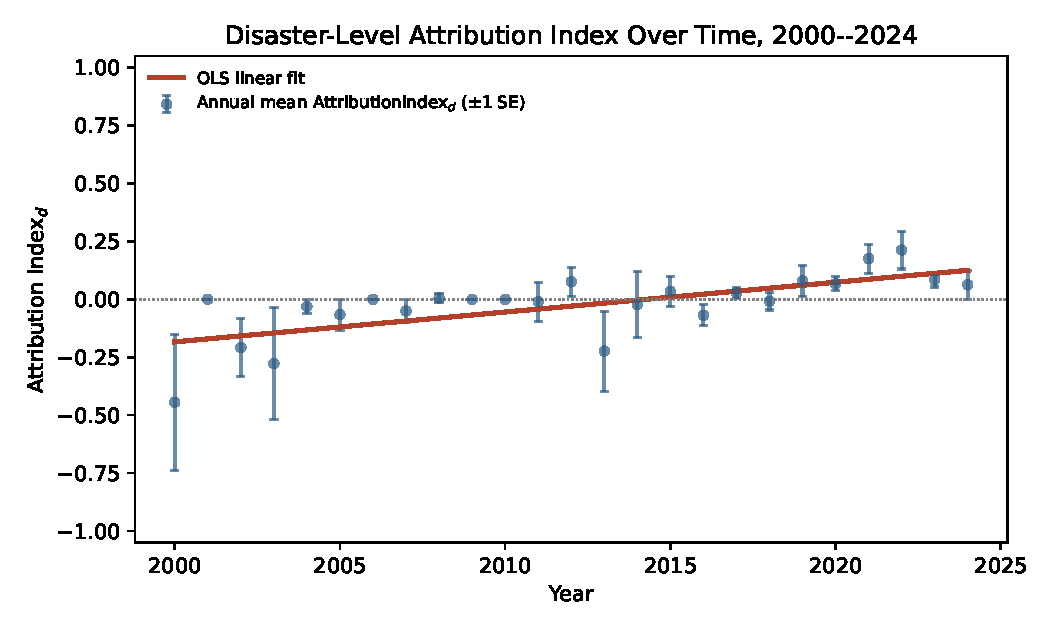
\includegraphics[width=0.8\textwidth]{figures/attribution_trend.pdf}
\caption{Attribution Index Over Time}
\label{fig:trend_over_time}
\end{figure}

\subsection{Variation by Geography}

TODO: Coastal vs.\ inland, red vs.\ blue states.

\subsection{Variation by Disaster Type and Severity}

TODO: Wildfires/hurricanes vs.\ floods/severe storms; cost as a
predictor of anthropogenic framing.

\subsection{Main Regression Results}

TODO: Table~\ref{tab:main_results}.

\begin{table}[ht]
\centering
\caption{Determinants of the Attribution Index}
\label{tab:main_results}
\begin{threeparttable}
\begin{tabular}{lccc}
\toprule
 & (1) & (2) & (3) \\
\midrule
TODO & & & \\
\bottomrule
\end{tabular}
\begin{tablenotes}
\small
\item Notes: TODO. Standard errors in parentheses.
\end{tablenotes}
\end{threeparttable}
\end{table}


% ===================================================================
\section{Robustness}
% ===================================================================

TODO: Alternative classifiers, sample restrictions (national vs.\
local outlets only), placebo checks.


% ===================================================================
\section{Discussion}
% ===================================================================

TODO: Interpret findings in light of climate communication, risk
perception, and policy implications discussed in the Introduction.


% ===================================================================
\section{Conclusion}
% ===================================================================

TODO: Summarize contribution, limitations, and directions for future
work.


% ===================================================================
\newpage
\begin{thebibliography}{99}

\bibitem[Landis and Koch(1977)]{landiskoch1977}
Landis, J.~R. and Koch, G.~G. (1977).
\newblock The Measurement of Observer Agreement for Categorical Data.
\newblock \emph{Biometrics}, 33(1):159--174.

\end{thebibliography}


% ===================================================================
\appendix
\section{Data Appendix}
% ===================================================================

\subsection{Disaster Event List}

TODO: Full list of 313 NOAA events with assigned states/regions and
PSE engine coverage.

\subsection{Newspaper Source List}

TODO: Description of the 19 Programmable Search Engines and their
domain coverage.

\subsection{Additional Tables and Figures}

TODO.

\end{document}
